\documentclass{article}

\usepackage[letterpaper,top=0.4in, left=0.8in, right=0.8in, bottom=1in]{geometry}

\usepackage{amsmath, amsfonts, amsthm, amssymb}
\usepackage{graphicx, float}
\usepackage{mathtools}
\usepackage{stackrel}
\usepackage{siunitx}
\usepackage{esdiff}
\usepackage{titlesec}
\usepackage{multicol}
\usepackage{vwcol}
\usepackage{interval}
\usepackage{afterpage}
\usepackage{tikz}
\usepackage{mdframed}
\usepackage{cancel}
\usepackage{tabularray}
\usepackage{empheq}
\usepackage[export]{adjustbox}

\usetikzlibrary{positioning}
\usetikzlibrary{angles,quotes}

\intervalconfig {
	soft open fences
}
\newcommand{\alignedintertext}[1]{%
	\noalign{%
		\vskip\belowdisplayshortskip
		\vtop{\hsize=\linewidth#1\par
		\expandafter}%
		\expandafter\prevdepth\the\prevdepth
	}%
}

\title{Progress on Problem Set \#40}
\author{Jayden Li}
\date{January 10, 2024}

\allowdisplaybreaks

\begin{document}

\fontsize{12pt}{12pt}\selectfont

\maketitle

\section*{Problem 1}
\begin{figure}[ht]
	\begin{minipage}[t]{0.55\linewidth}
		\centering
		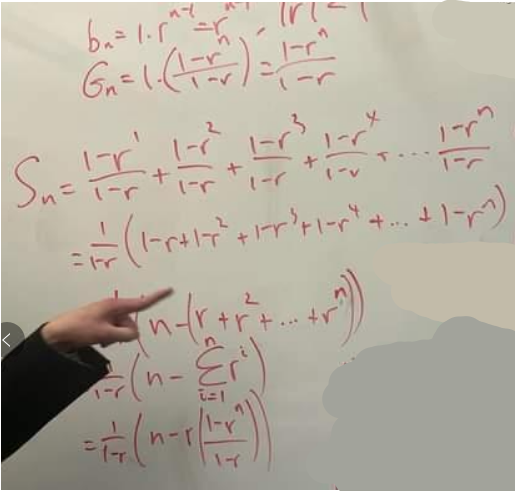
\includegraphics[width=\linewidth, valign=t]{q1.png}
	\end{minipage}
	\begin{minipage}[t]{0.4\linewidth}
	\setlength{\abovedisplayskip}{0pt}
	\begin{align*}
		a_n&=a_1+d(n-1) \\
		&=1+d(n-1) \\
		A_n&=\sum_{i=1}^{n}a_i \\
		&=\frac{(1+1+d(n-1))n}{2} \\
		&=\frac{(2+dn-d)n}{2} \\
		\\
		S_n&=\frac{1}{1-r}\left(n-r\left(\frac{1-r^n}{1-r}\right)
			\right) \\
		&=\frac{n}{1-r}-\frac{r(1-r^n)}{(1-r)^2} \\
		&=\frac{n(1-r)}{(1-r)(1-r)}-\frac{r(1-r^n)}{(1-r)(1-r)} \\
		&=\frac{n-nr-r(1-r^n)}{(1-r)^2}
	\end{align*}
	\end{minipage}
\end{figure}
\begin{align*}
	\lim_{n\to\infty}\left(\frac{A_n}{n}-S_n\right)&=1 \\
	\lim_{n\to\infty}\left(\frac{(2+dn-d)n}{2n}-\frac{1}{1-r}
		\left(n-r\left(\frac{1-r^n}{1-r}\right)\right)\right)&=1 \\
	\lim_{n\to\infty}\left(\frac{2+dn-d}{2}-
		\frac{n-nr-r(1-\cancelto{0}{r^n})}{(1-r)^2}\right)&=1 \\
	\lim_{n\to\infty}\frac{2+dn-d}{2}-
		\lim_{n\to\infty}\frac{n-nr-r}{(1-r)^2}&=1 \\
	\lim_{n\to\infty}\frac{2+dn-d}{2}-1
		&=\lim_{n\to\infty}\frac{n-nr-r}{(1-r)^2} \\
	2(1-r)^2\cdot\lim_{n\to\infty}\frac{dn-d}{2}&=2(1-r)^2\cdot
		\lim_{n\to\infty}\frac{n-nr-r}{(1-r)^2} \\
	\lim_{n\to\infty}\left((dn-d)(1-r)^2\right)&=
		\lim_{n\to\infty}2\left(n-nr-r\right) \\
	\lim_{n\to\infty}\left((dn-d)(1-2r+r^2)\right)&=
		\lim_{n\to\infty}2\left(n-nr-r+r^{n+1}\right) \\
	\lim_{n\to\infty}\left(dn-2rdn+r^2dn-d+2rd-dr^2\right)&=
		\lim_{n\to\infty}\left(2n-2nr-2r+2r^{n+1}\right) \\
	\lim_{n\to\infty}\left(dn-2rdn+r^2dn-2n+2nr\right)&=
		\lim_{n\to\infty}\left(-2r+\cancelto{0}{2r^{n+1}}+d
		-2rd+dr^2\right) \\
	\lim_{n\to\infty}n\left(d-2rd+r^2d-2+2r\right)&=
		-2r+d-2rd+dr^2 \\
\end{align*}
RHS is a real (and therefore bounded) value so LHS must also
converge. This means that:
\begin{equation*}
	d-2rd+r^2d-2+2r=0=-2r+d-2rd+dr^2
\end{equation*}
\begin{align*}
	\cancel{d-2rd+dr^2}-2+2r&=-2r+\cancel{d-2rd+dr^2} \\
	2r-2&=-2r \\
	4r&=2 \\
	\Aboxed{r&=\frac{1}{2}}
\end{align*}
\begin{align*}
	\lim_{n\to\infty}\left(\frac{(2+dn-d)n}{2n}-\frac{1}{1-r}
		\left(n-r\left(\frac{1-r^n}{1-r}\right)\right)\right)&=1 \\
	\lim_{n\to\infty}\left(\frac{2+dn-d}{2}-\frac{1}{1
		-\frac{1}{2}}\left(n-\left(\frac{1}{2}\right)\left(
		\frac{1-\left(\frac{1}{2}\right)^n}{1-\frac{1}{2}}\right)
		\right)\right)&=1 \\
	\lim_{n\to\infty}\left(\frac{2+dn-d}{2}-2\left(n-\left(\frac{1}{2}
		\right)\left(\frac{1-0}{\frac{1}{2}}\right)\right)\right)&=1 \\
	\lim_{n\to\infty}\left(\frac{2+dn-d}{2}-2\left(n-1\right)
		\right)&=1 \\
	2\lim_{n\to\infty}\left(\frac{2+dn-d}{2}-2n+2 \right)&=2 \\
	\lim_{n\to\infty}(2+dn-d-4n+4)&=2 \\
	\lim_{n\to\infty}(dn-d-4n)&=-4 \\
	\lim_{n\to\infty}n(d-4)&=d-4 \\
	d-4&=d-4=0 \\
	\Aboxed{d&=4}
\end{align*}

\pagebreak
\section*{Problem 2}
\begin{empheq}[left=\empheqlbrace]{gather}
	\displaystyle 2\sum_{i=0}^\infty(\log_2p)^i=
		\sum_{k=1}^\infty(1+q)^{-k} \\
	\displaystyle \sum_{k=1}^1(1+q)^{-k}-
		\sum_{i=0}^1(\log_2p)^i=\frac{7}{5}
\end{empheq}
\centering
\begin{minipage}[t]{0.57\linewidth}
\begin{align*}
	\sum_{i=0}^1(\log_2p)^i+\frac{7}{5}&=\sum_{k=1}^1(1+q)^{-k} \\
	(\log_2p)^0+(\log_2p)^1+\frac{7}{5}&=(1+q)^{-1} \\
	\frac{5}{5}+\log_2p+\frac{7}{5}&=\frac{1}{1+q} \\
	\log_2p+\frac{12}{5}&=\frac{1}{1+q} \\
	2^{\log_2p+\frac{12}{5}}&=2^{\frac{1}{1+q}} \\
	2^{\log_2p}\cdot2^{\frac{12}{5}}&=2^{\frac{1}{1+q}} \\
	p2^{\frac{12}{5}}&=2^{\frac{1}{1+q}} \\
	p&=\frac{2^{\frac{1}{1+q}}}{2^{\frac{12}{5}}} \\
	p&=2^{\frac{1}{1+q}-\frac{12}{5}} \\
\end{align*}
\textbf{Case 1.}
\begin{minipage}[t]{0.28\linewidth}
$\begin{aligned}[t]
	q&=-\frac{4}{5} \\
	p&=2^{\frac{1}{-\frac{4}{5}}-\frac{12}{5}} \\
	&=2^{-\frac{5}{4}-\frac{12}{5}} \\
	&=2^{-\frac{25}{20}-\frac{48}{20}} \\
	&=2^{-\frac{73}{20}} \\
\end{aligned}$
\end{minipage}
\begin{minipage}[t]{0.29\linewidth}
$\begin{aligned}[t]
	&2\sum_{i=0}^\infty(\log_2p)^i \\
	=\,&2\sum_{i=0}^\infty\left(-\frac{73}{20}\right)^i
\end{aligned}$
\end{minipage} \\
This series does not converge as
$\left|-\dfrac{73}{20}\right|\geq1$.

\textbf{Case 2.}
\begin{minipage}[t]{0.28\linewidth}
$\begin{aligned}[t]
	q&=\frac{3}{2} \\
	p&=2^{\frac{1}{\frac{3}{2}}-\frac{12}{5}} \\
	&=2^{\frac{2}{3}-\frac{12}{5}} \\
	&=2^{-\frac{10}{15}-\frac{36}{15}} \\
	&=2^{-\frac{26}{15}} \\
\end{aligned}$
\end{minipage}
\begin{minipage}[t]{0.29\linewidth}
$\begin{aligned}[t]
	&2\sum_{i=0}^\infty(\log_2p)^i \\
	=\,&2\sum_{i=0}^\infty\left(-\frac{26}{15}\right)^i
\end{aligned}$
\end{minipage} \\
This series does not converge as
$\left|-\dfrac{26}{15}\right|\geq1$.
\end{minipage}
\begin{minipage}[t]{0.42\linewidth}
\begin{align*}
	2\sum_{i=0}^\infty(\log_2p)^i&=\sum_{k=1}^\infty(1+q)^{-k} \\
	2\sum_{i=0}^\infty\left(\log_2\left(2^{\frac{1}{1+q}-
		\frac{12}{5}}\right)\right)^i&=
		\sum_{k=1}^\infty\frac{1}{(1+q)^k} \\
	2\sum_{i=0}^\infty\left(\frac{1}{1+q}-\frac{12}{5}\right)^i
		&=\sum_{k=1}^\infty\left(\frac{1}{1+q}\right)^k \\
	2\cdot\frac{\left(\frac{1}{1+q}-\frac{12}{5}\right)^0}
		{1-\left(\frac{1}{1+q}-\frac{12}{5}\right)}&=
		\frac{\left(\frac{1}{1+q}\right)^1}{1-\left(
		\frac{1}{1+q}\right)} \\
	\frac{2}{1-\frac{1}{1+q}+\frac{12}{5}}&=
		\frac{\frac{1}{1+q}}{1-\frac{1}{1+q}} \\
	\frac{2}{\frac{17}{5}-\frac{1}{1+q}}&=
		\frac{\frac{1}{1+q}}{\frac{1+q}{1+q}-\frac{1}{1+q}} \\
	\frac{2}{\frac{17(1+q)}{5(1+q)}-\frac{5}{5(1+q)}}&=
		\frac{\frac{1}{1+q}}{\frac{q}{1+q}} \\
	\frac{2}{\frac{17+17q-5}{5+5q}}&=\frac{1}{q} \\
	2\cdot\frac{5+5q}{17+17q-5}&=\frac{1}{q} \\
	\frac{10+10q}{17+17q-5}&=\frac{1}{q} \\
	10q+10q^2&=17+17q-5 \\
	10q^2-7q-12&=0 \\
	10q^2-15q+8q-12&=0 \\
	5q(2q-3)+4(2q-3)&=0 \\
	(5q+4)(2q-3)&=0
	\intertext{\centering$\displaystyle q=-\frac{4}{5},\frac{3}{2}$}
\end{align*}
\centering
\boxed{\text{No Solutions.}}
\end{minipage}
\flushleft

\pagebreak
\section*{Problem 3}

\begin{gather*}
	\sum_{k=1}^{\infty}\left(\frac{2x-1}{x+2}\right)^k=R \\
	-1<\frac{2x-1}{x+2}<1
\end{gather*}
\centering
\begin{minipage}[t]{0.45\linewidth}
\begin{align*}
	-1<\frac{2x-1}{x+2} \\
	\frac{2x-1}{x+2}+\frac{x+2}{x+2}>0 \\
	\frac{3x-1}{x+2}>0 \\
\end{align*}
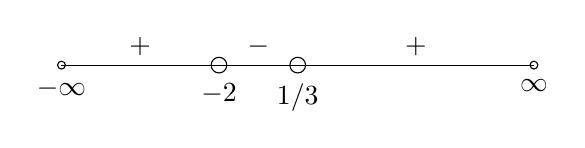
\begin{tikzpicture}	
	\draw
	(0,0) node[circle,draw,inner sep=1pt,label=below:$-\infty$](){}
 -- (2,0) node[circle,draw,inner sep=2pt,label=below:$-2$](){} node[midway,above]{$+$}
 -- (3,0) node[circle,draw,inner sep=2pt,label=below:$1/3$](){} node[midway,above]{$-$}
 -- (6,0) node[circle,draw,inner sep=1pt,label=below:$\infty$](){} node[midway,above]{$+$};
\end{tikzpicture}
\end{minipage}
\begin{minipage}[t]{0.45\linewidth}
\begin{align*}
	\frac{2x-1}{x+2}<1 \\
	\frac{2x-1}{x+2}-\frac{x+2}{x+2}<0 \\
	\frac{x-3}{x+2}<0 \\
\end{align*}
\begin{tikzpicture}	
	\draw
	(0,0) node[circle,draw,inner sep=1pt,label=below:$-\infty$](){}
 -- (2,0) node[circle,draw,inner sep=2pt,label=below:$-2$](){} node[midway,above]{$+$}
 -- (4,0) node[circle,draw,inner sep=2pt,label=below:$3$](){} node[midway,above]{$-$}
 -- (6,0) node[circle,draw,inner sep=1pt,label=below:$\infty$](){} node[midway,above]{$+$};
\end{tikzpicture}
\end{minipage}
\flushleft
\[
	x\in\interval[scaled,open left,open right]{-\frac{1}{3}}{3}
\]

\begin{align*}
	\sum_{k=1}^{\infty}\left(\frac{2x-1}{x+2}\right)^k=
		\frac{\frac{2x-1}{x+2}}{1-\frac{2x-1}{x+2}}&=R \\
	\frac{\frac{2x-1}{x+2}}{\frac{x+2}{x+2}-\frac{2x-1}{x+2}}&=R \\
	\frac{2x-1}{\cancel{(x+2)}\cdot\frac{x+2-2x+1}{\cancel{x+2}}}&=R \\
	\frac{2x-1}{-x+3}&=R \\
\end{align*}

The range of $R$ is the range of $\dfrac{2x-1}{-x+3}$ where
$x\in\interval[scaled,open left,open right]{-\dfrac{1}{3}}{3}$.

\pagebreak
\section*{Problem 6}
Let $r$ be the common ratio.

\centering
\begin{minipage}[t]{0.42\linewidth}
\begin{align*}
	\sin\theta&=\frac{R_{n+1}}{x} \\
	\sin\theta&=\frac{R_n}{x+R_n+R_{n+1}} \\
	\\
	\sin\theta&=\frac{rR_n}{x} \\
	\sin\theta&=\frac{R_n}{x+R_n+rR_n} \\
	\\
	\frac{rR_n}{x}&=\frac{R_n}{x+R_n+rR_n} \\
	\frac{r}{x}&=\frac{1}{x+R_n+rR_n} \\
	rx+rR_n+r^2R_n&=x \\
	R_n(r+r^2)&=x-rx \\
	R_n&=\frac{x(1-r)}{r(1+r)} \\
\end{align*}

\begin{align*}
	\sum_{k=1}^{\infty}R_k&=\frac{R_1}{1-r} \\
	2\pi&=\frac{\frac{4}{3}}{1-\frac{1-\sin\theta}{\sin\theta+1}} \\
	6\pi&=\frac{4}{\frac{\sin\theta+1}{\sin\theta+1}-
		\frac{1-\sin\theta}{\sin\theta+1}} \\
	6\pi&=\frac{4}{\frac{2\sin\theta}{\sin\theta+1}} \\
	6\pi&=4\cdot\frac{\sin\theta+1}{2\sin\theta} \\
	12\pi\sin\theta&=4\sin\theta+4 \\
	3\pi\sin\theta-\sin\theta&=1 \\
	\sin\left(\theta\right)\left(3\pi-1\right)&=1 \\
	\sin\theta&=\frac{1}{3\pi-1} \\
	\Aboxed{\theta&=\arcsin\left(\frac{1}{3\pi-1}\right)}
\end{align*}
\end{minipage}
\begin{minipage}[t]{0.56\linewidth}
\setlength{\abovedisplayskip}{0pt}
\begin{align*}
	\sin\theta&=\frac{r\cdot\frac{x(1-r)}{r(1+r)}}{x} \\
	\sin\theta&=\frac{\frac{x(1-r)}{r(1+r)}}
		{x+\frac{x(1-r)}{r(1+r)}+r\cdot\frac{x(1-r)}{r(1+r)}} \\
	\\
	\sin\theta&=\frac{1-r}{1+r} \\
	\sin\theta&=\frac{\frac{x(1-r)}{r(1+r)}}{\frac{xr(1+r)}
		{r(1+r)}+\frac{x(1-r)}{r(1+r)}+\frac{rx(1-r)}{r(1+r)}} \\
	\sin\theta&=\frac{x(1-r)}{xr(1+r)+x(1-r)+rx(1-r)} \\
	\sin\theta&=\frac{1-r}{r(1+r)+(1-r)+r(1-r)} \\
	\sin\theta&=\frac{1-r}{r+r^2+1-r+r-r^2} \\
	\sin\theta&=\frac{1-r}{r+1} \\
	r\sin\theta+\sin\theta&=1-r \\
	r\sin\theta+r&=1-\sin\theta \\
	r(\sin\theta+1)&=1-\sin\theta \\
	r&=\frac{1-\sin\theta}{\sin\theta+1}
\end{align*}
\end{minipage}

\end{document}
